\documentclass[UTF8]{ctexart}
\usepackage{dirtree}
\usepackage{listings}
\usepackage{xcolor}
\usepackage{graphicx}
\usepackage{enumerate}
\usepackage[a4paper]{geometry} 
\usepackage{amsmath,amsthm,mathtools}
\usepackage{mathtools}
\usepackage{diagbox}
\usepackage{multirow,makecell}
\usepackage{float}
\usepackage{url}
\usepackage[nottoc]{tocbibind}
\usepackage{float}
\newcommand{\refe}[1]{Eq.\ref{#1}}
\newcommand{\reft}[1]{Theory.\ref{#1}\ }
\newcommand{\reff}[1]{图\ref{#1}\ }
\newtheorem{theorem}{Theory}[section]
\geometry{bottom=2cm,left=1cm,right=1cm}

%插入代码样式设置
\lstset{
 columns=fixed,
 numbers=left,                                        % 在左侧显示行号
 numberstyle=\tiny\color{gray},                       % 设定行号格式
 basicstyle=\small\ttfamily,
 frame=none,                                          % 不显示背景边框
 backgroundcolor=\color[RGB]{245,245,244},            % 设定背景颜色
 keywordstyle=\color[RGB]{40,40,255},                 % 设定关键字颜色
 numberstyle=\footnotesize\color{darkgray},           
 commentstyle=\color{gray}\ttfamily,                  % 设置代码注释的格式
 stringstyle=\rmfamily\slshape\color[RGB]{128,0,0},   % 设置字符串格式
 showstringspaces=false,
 breaklines=true,
 language=python
}

\title{实验一:基于文件系统的学生选课管理}
\author{张配天-2018202180}

\begin{document}
    \maketitle
    \tableofcontents
    \clearpage
    \section{实验环境}
    \begin{itemize}
        \item cpu:AMD4800HS;gpu:RTX2060mq
        \item os:win10,wsl
        \item 语言:python
        \item 工具:vscode
    \end{itemize}
    \section{实验步骤}
    \subsection{文件组织}
    \begin{itemize}
        \item lab1.csv:按照word中的说明,每一列分别为:学号、姓名、性别、年龄、专业、课程名、课程号、课程学分、课程成绩;
        每一行为一条选课信息;
        \item \textbf{编号不可重复,姓名可重复;}
    \end{itemize}
    \subsection{数据结构}
    \begin{itemize}
        \item 为了最快地进行查找,使用字典存储数据;
        \item 课程和学生都有查找需求,因此维护两个字典,分别存放课程和学生;
        \item 因为可以通过编号或名称两项作为关键字,因此额外维护两个字典,用于映射课程名到课程编号、学生名到学生编号;
        \item \textbf{将四个字典存储到文件,}每次读取,作为加载数据;
        \item \textbf{可以从csv中添加新的选课记录,更新字典,更新文件;}
        \item 数据规模不大,因此牺牲一些空间,在\textbf{加载数据时计算学生平均分和课程平均分},直接存入(更新)数据结构;
        \item \textbf{每次删除数据和修改数据时需要动态修改两个字典中的对应成绩、平均成绩、学分;}
    \end{itemize}
    \par 综上,实现数据结构如下:
    \begin{lstlisting}
        dict students = {
            str stuID,              #学号
            str stuNM,              #学生姓名
            str gender,             #学生性别
            str age,                #学生年龄
            str major,              #学生专业
            int credit,             #学生学分
            float average,          #学生平均分
            dict grades = {         #学生选的课程及其分数
                curID:str grade     #课程号,对应分数
            }
        }
        dict curriculums = {             
            str curID,              #课程号
            str curNM,              #课程名
            int credit,             #课程学分
            float average,          #课程平均分
            dict grades:{           #选这门课的学生及其分数
                stuID:str grade     #学号,对应分数
            }
        }
        dict stuNM2id = {           #将学生名映射到学号
            stuNM:[stuIDs]           
        }
        dict curNM2id = {           #将课程名映射到课程号
            curNM:[curIDs]           
        }
    \end{lstlisting}
    \subsection{算法}
    \begin{itemize}
        \item 输入字符串,使用正则将其解析为查删改的命令,使用if...else语句判断各种输入的情况,执行对应操作;
        \item 利用字典的哈希属性进行快速查询,使用del关键字删除相应学生选课记录(删除学生数据结构中其对应课程,删除课程数据结构中其对应学生);
        \item 从零开始加载数据,构成四个字典;在四个字典的基础上,通过if来对比新的记录是否为\textbf{新的学生选了新的课程}、\textbf{已有的学生选了新的课程}还是\textbf{已有的学生选了已有的课程(重复的数据)},进行添加数据、更新字典;
        \item 通过删改学生成绩导致的平均成绩修改时,根据改动的成绩$\delta$来进行计算,减少运算量;
    \end{itemize}
    \section{实验结果}
    \subsection{查询}
    \begin{enumerate}
        \item 根据学号查找学生:
        \begin{figure}[H]
            \centering
            
\includegraphics[width=12cm]{resources/1.png}
        \end{figure}
        \item 根据姓名查找学生:
        \begin{figure}[H]
            \centering
            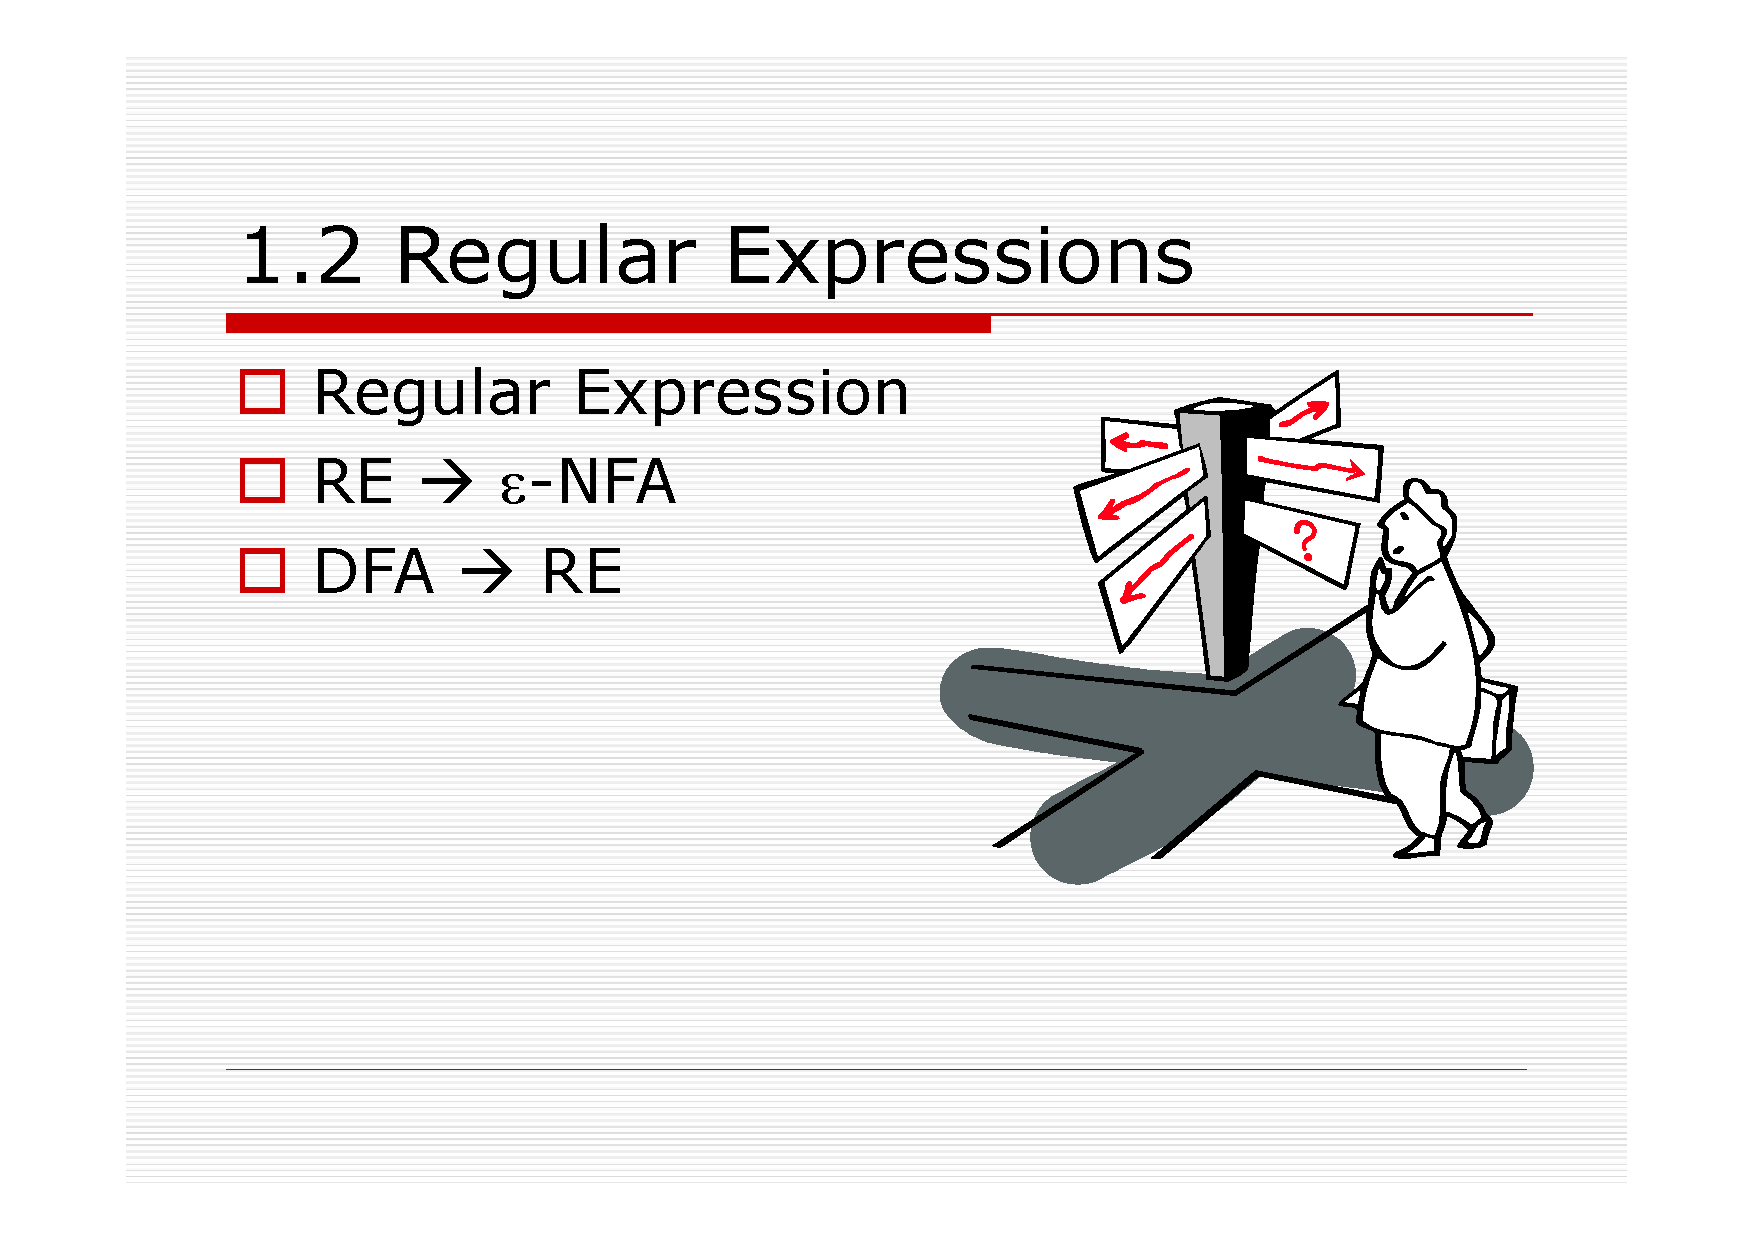
\includegraphics[width=12cm]{resources/2.png}
        \end{figure}
        \item 根据编号查找课程:
        \begin{figure}[H]
            \centering
            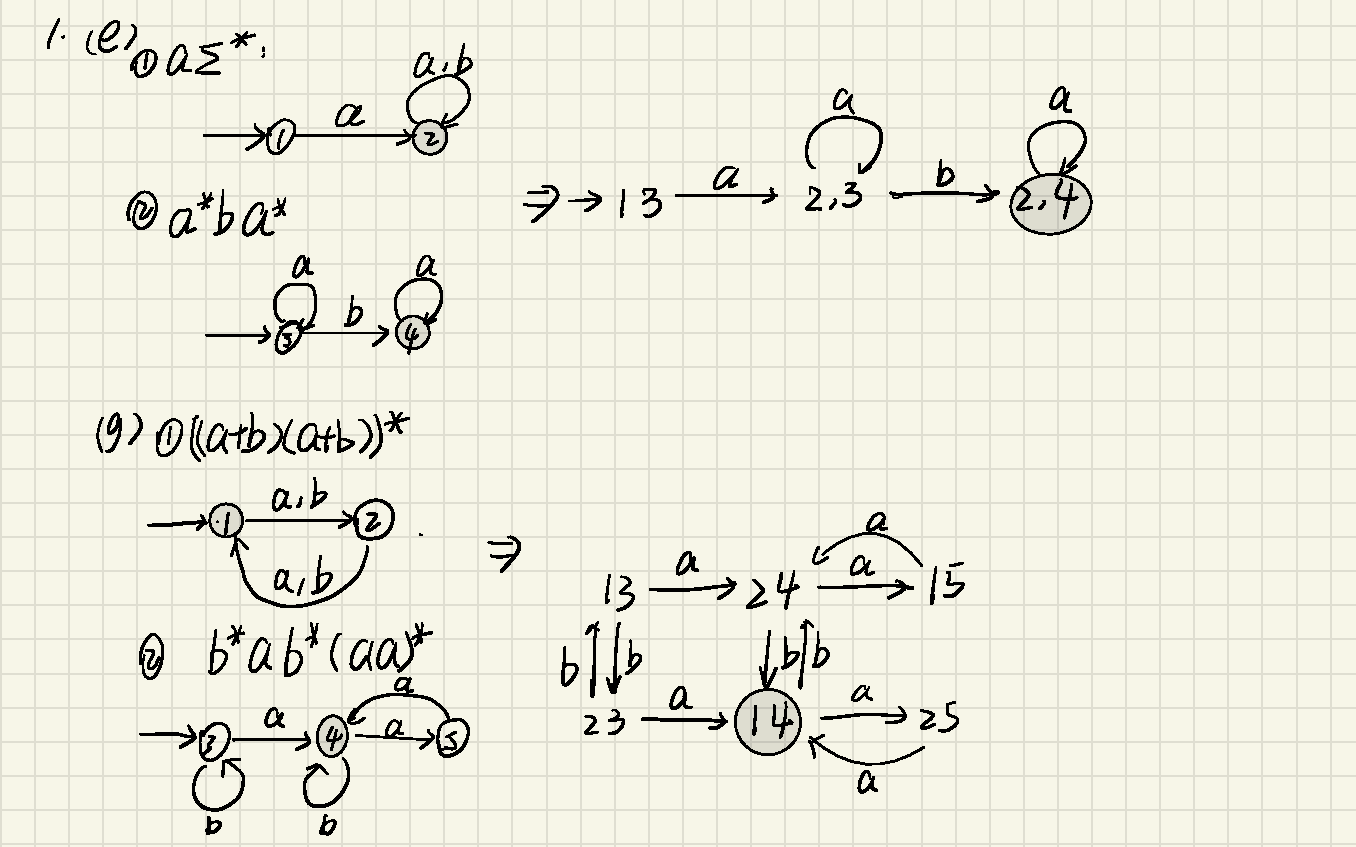
\includegraphics[width=12cm]{resources/3.png}
        \end{figure}
        \item 根据名称查找课程:
        \begin{figure}[H]
            \centering
            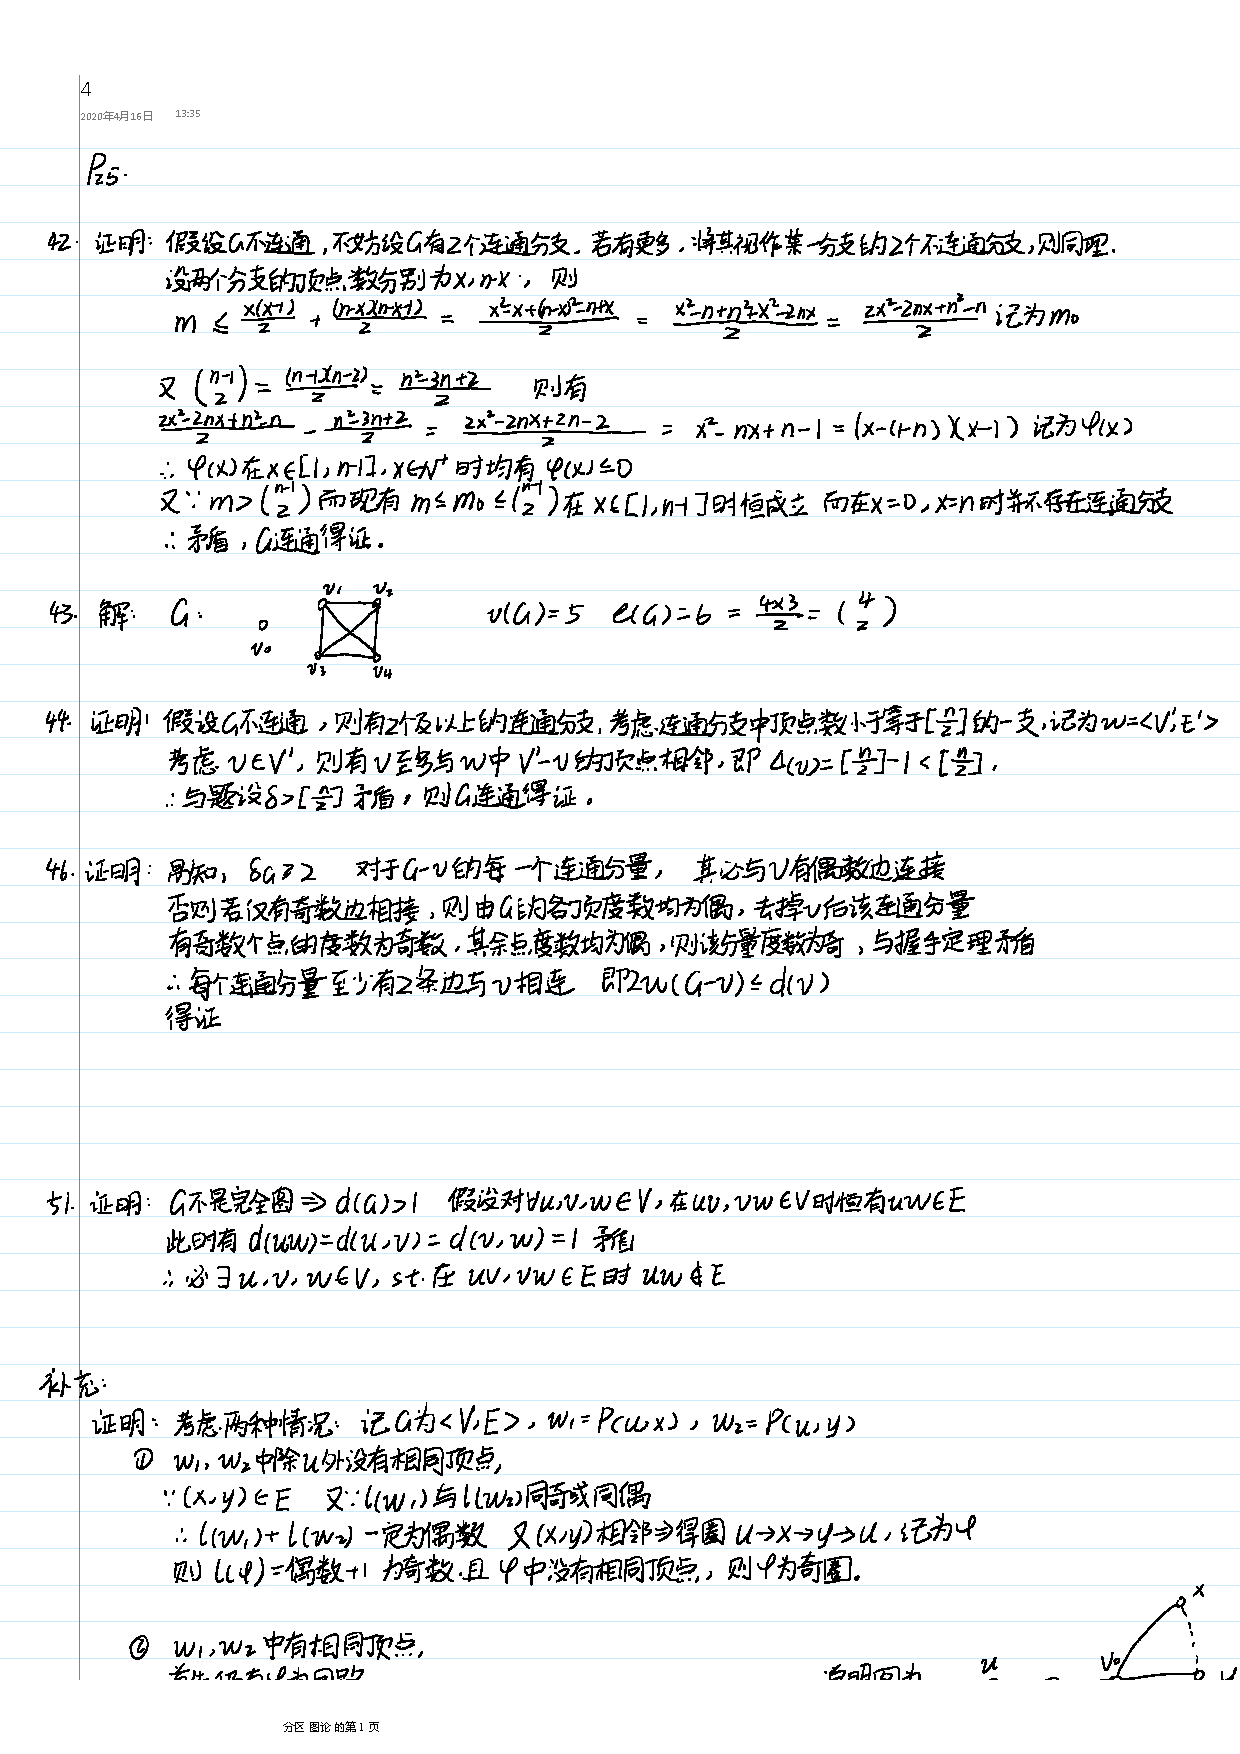
\includegraphics[width=12cm]{resources/4.png}
        \end{figure}
        \item 根据学号查找学生的平均分:
        \begin{figure}[H]
            \centering
            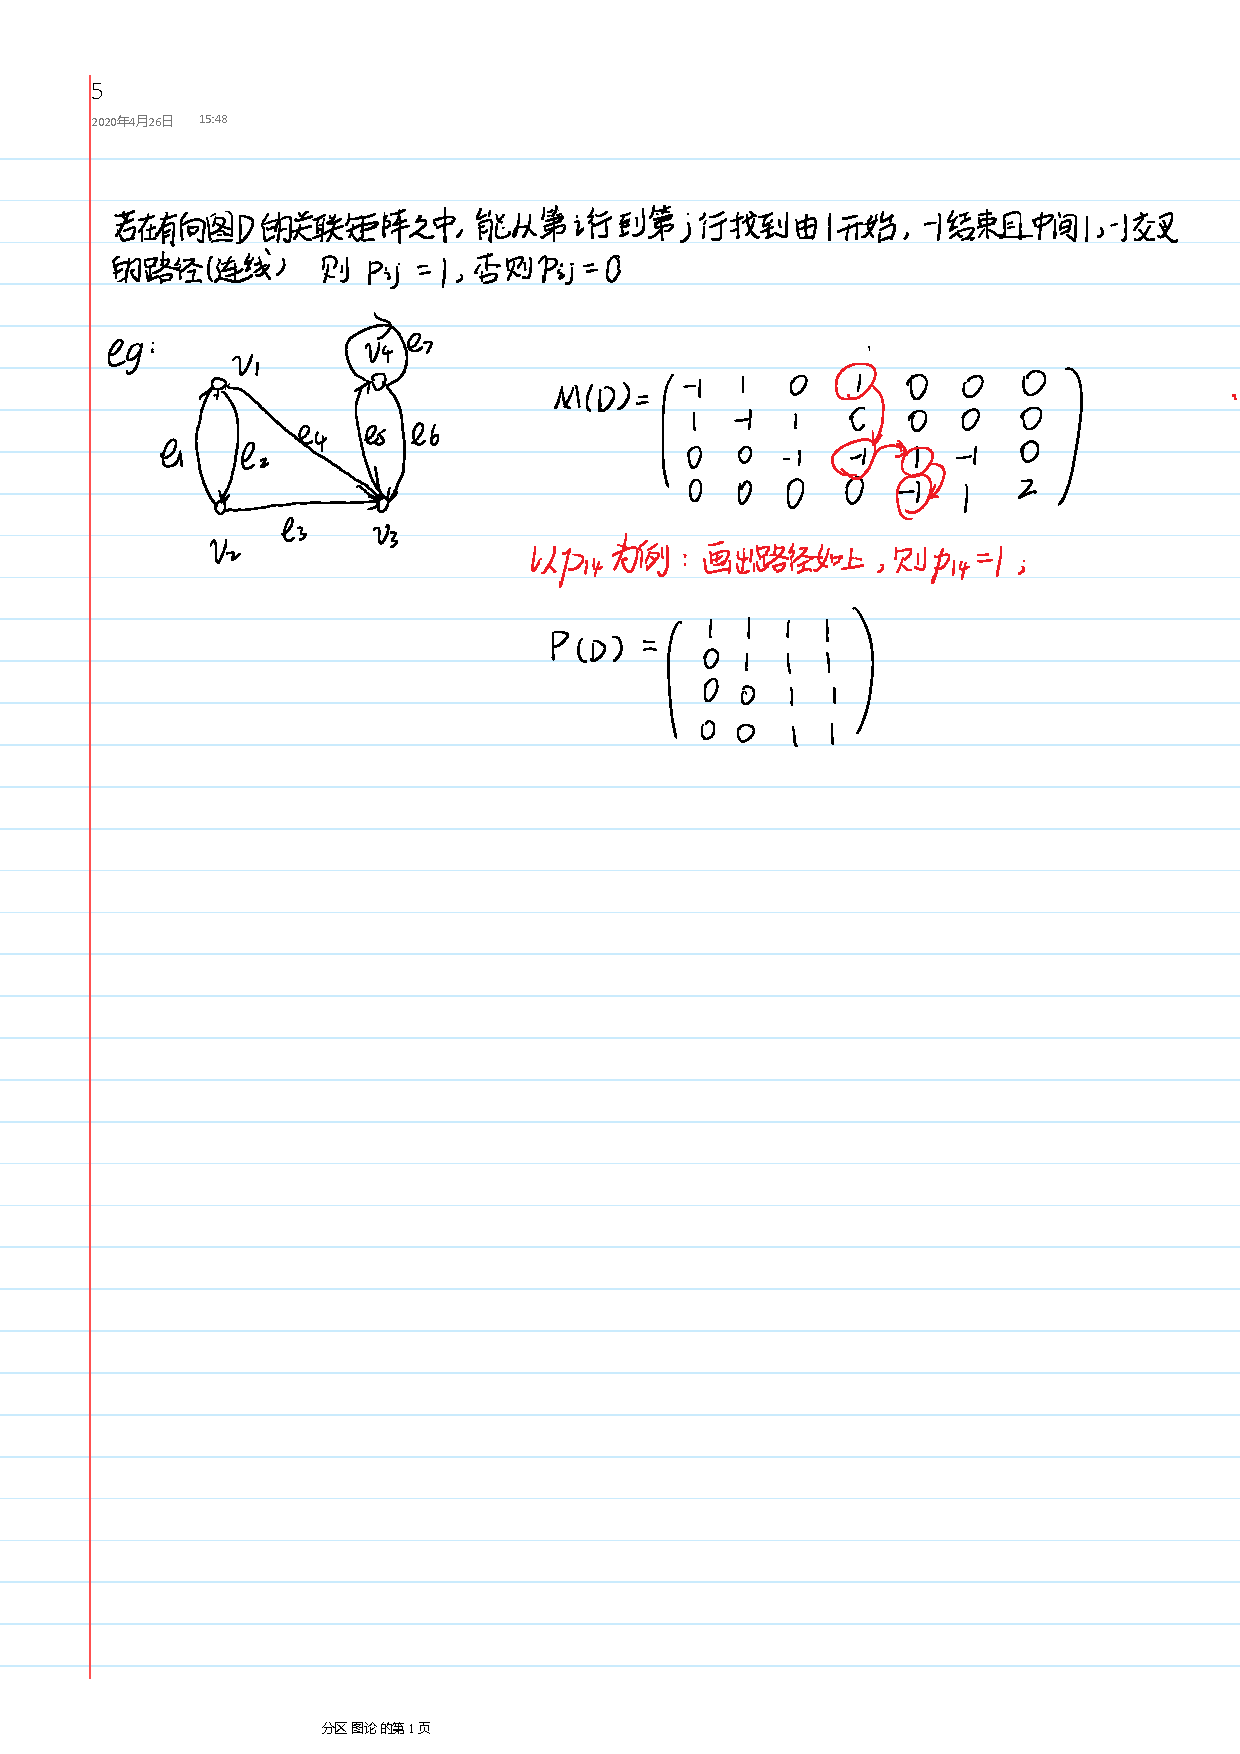
\includegraphics[width=12cm]{resources/5.png}
        \end{figure}
        \item 根据编号查找课程的平均分:
        \begin{figure}[H]
            \centering
            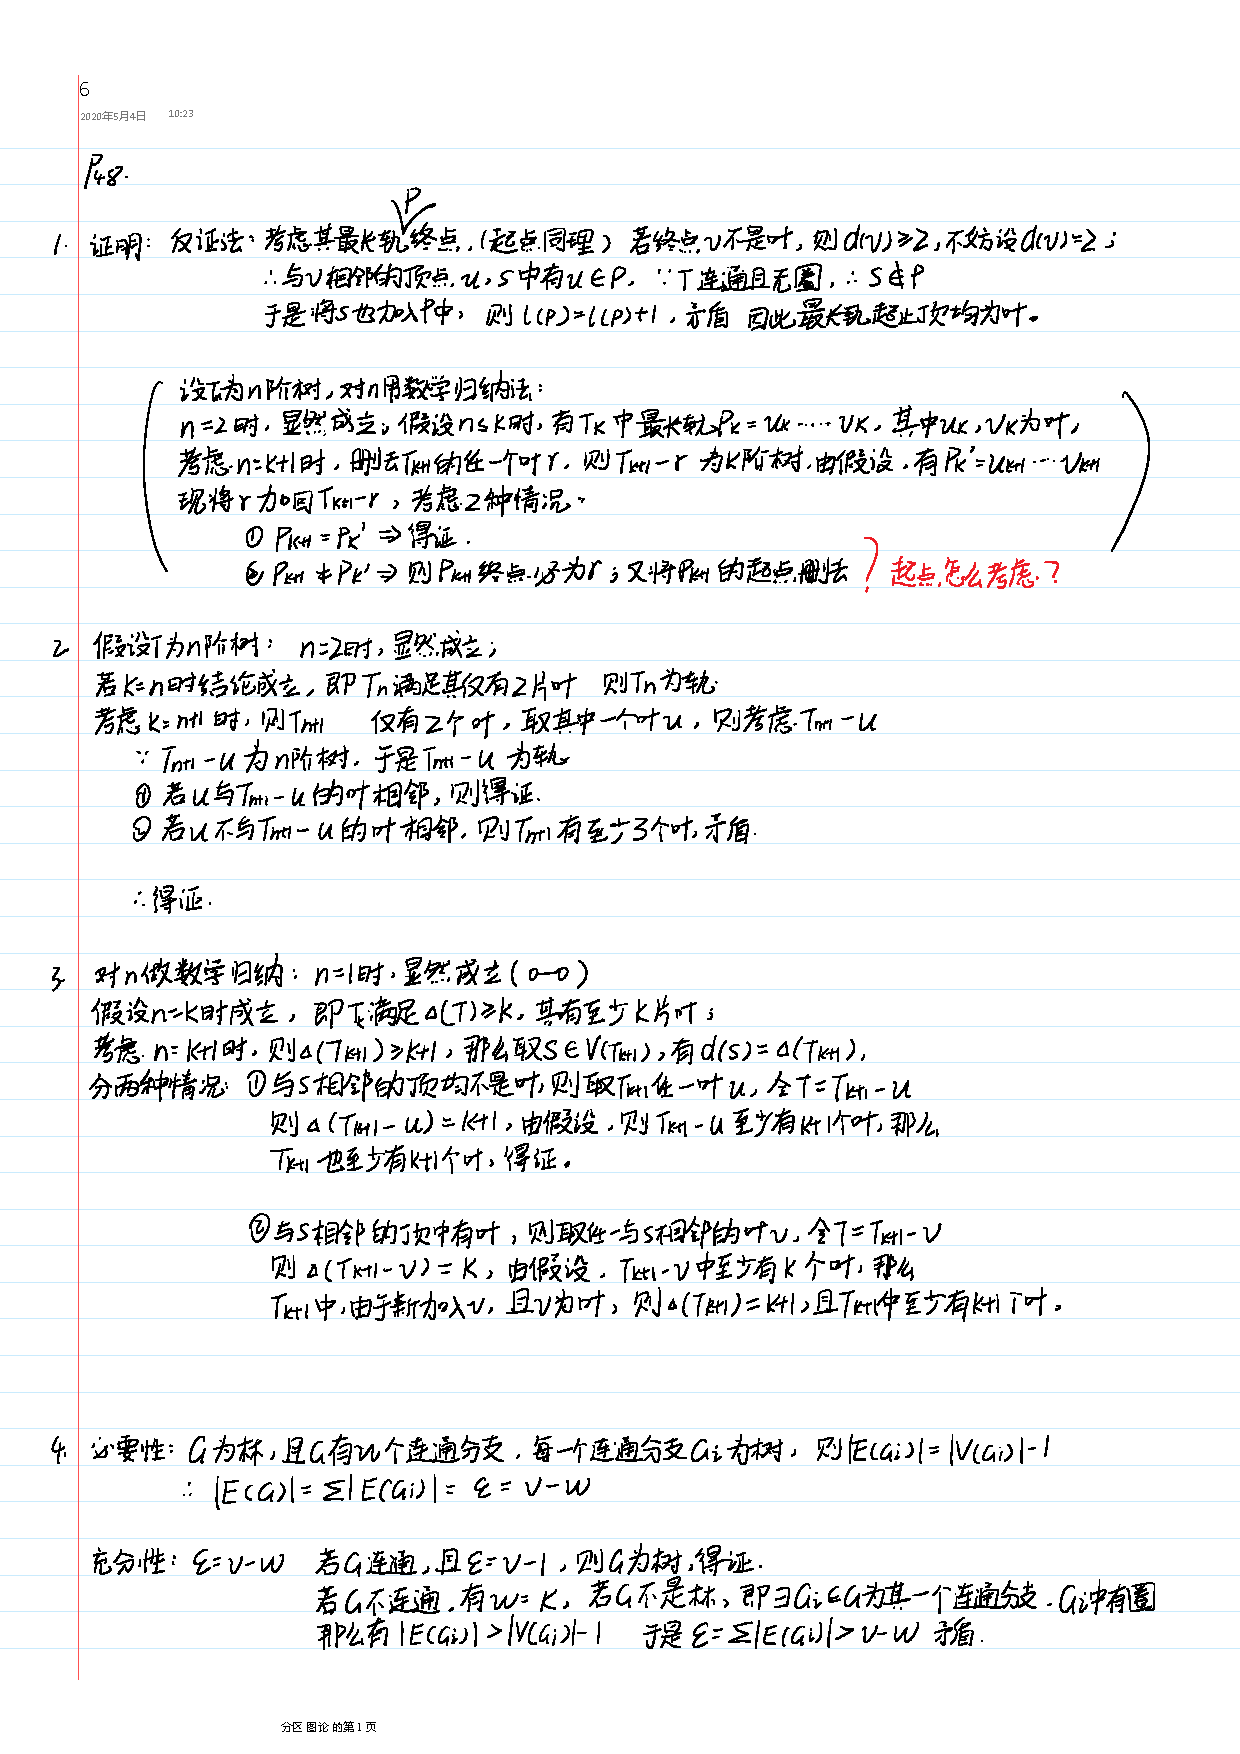
\includegraphics[width=12cm]{resources/6.png}
        \end{figure}
        \item 根据学号查找学生选修的课程数;
        \begin{figure}[H]
            \centering
            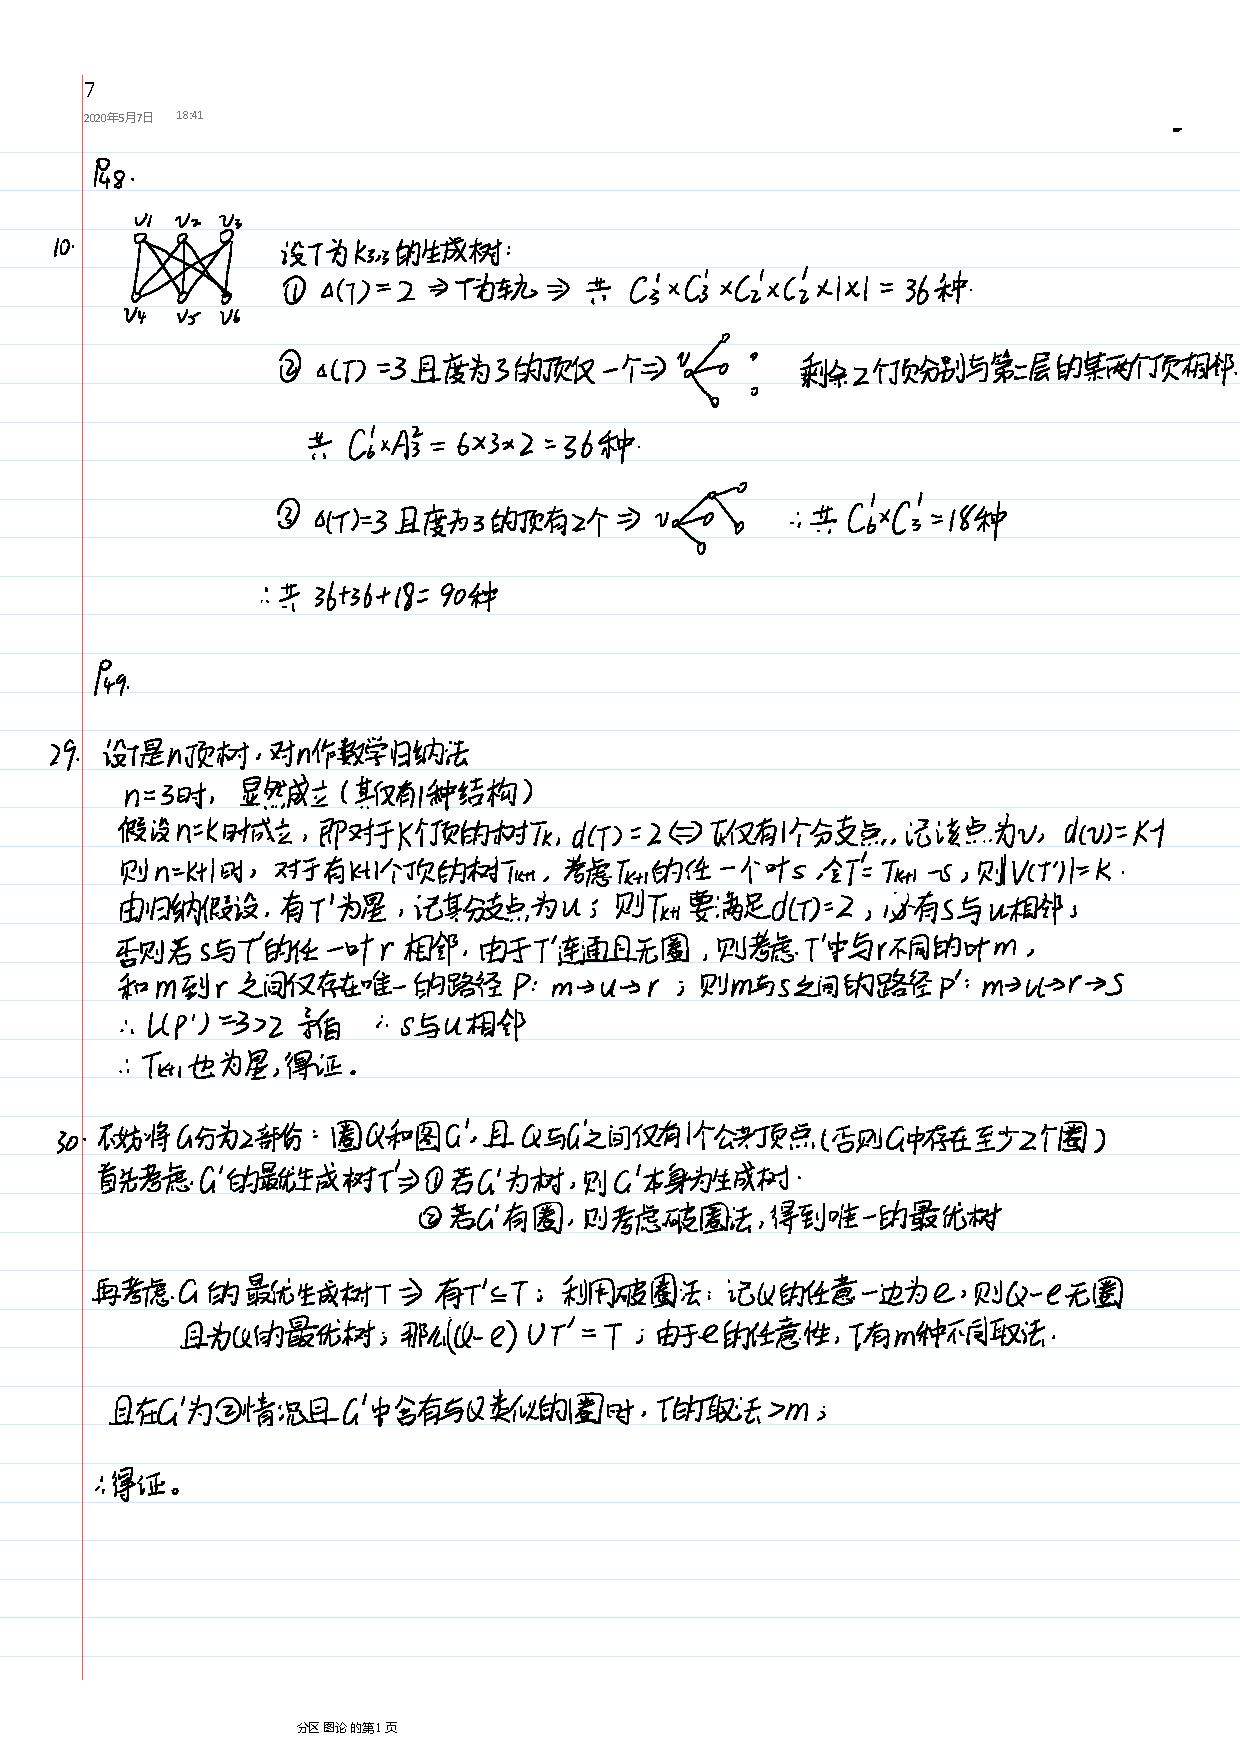
\includegraphics[width=12cm]{resources/7.png}
        \end{figure}
    \end{enumerate}
    \subsection{删改}
    \begin{enumerate}
        \item 根据学号和课程编号删除选课记录:
        \begin{figure}[H]
            \centering
            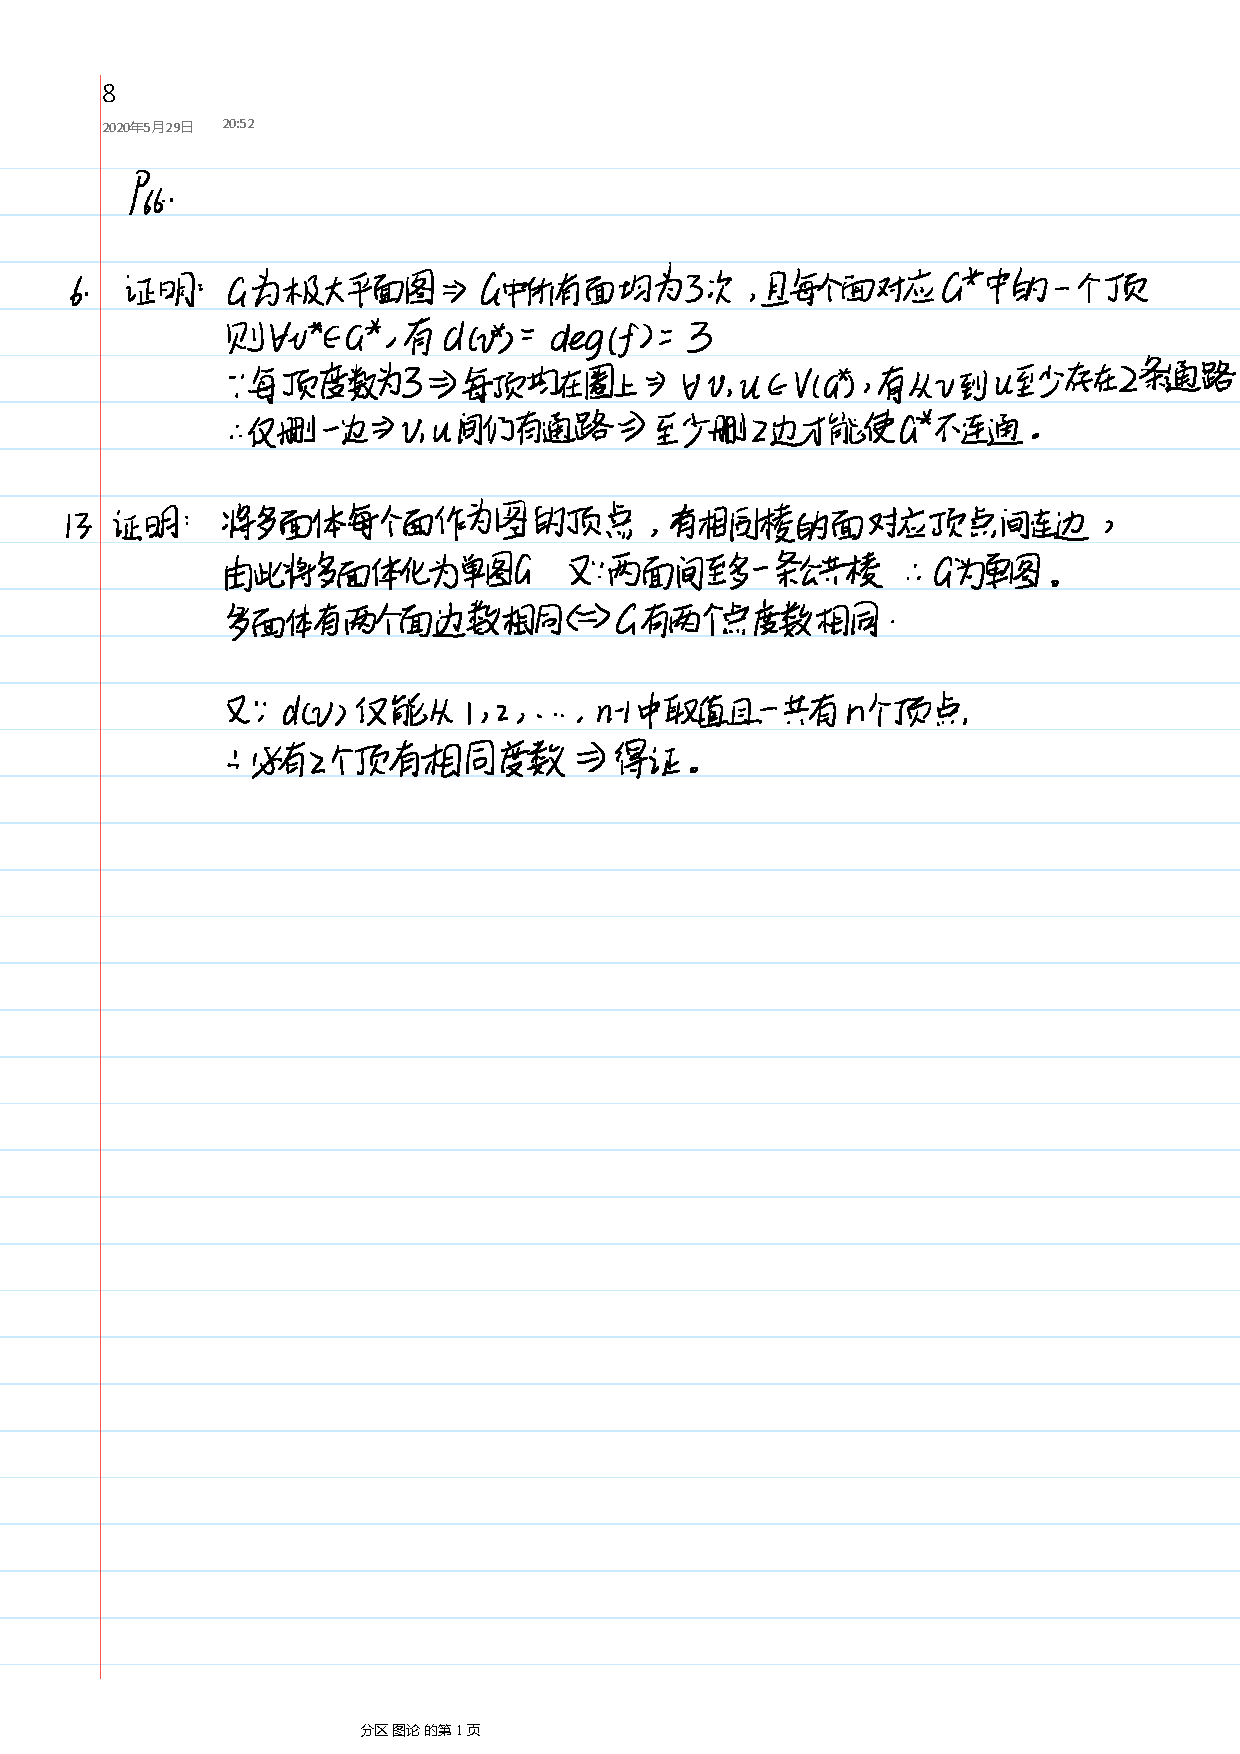
\includegraphics[width=12cm]{resources/8.png}
        \end{figure}
        \item 根据学号和课程编号修改学生成绩:
        \begin{figure}[H]
            \centering
            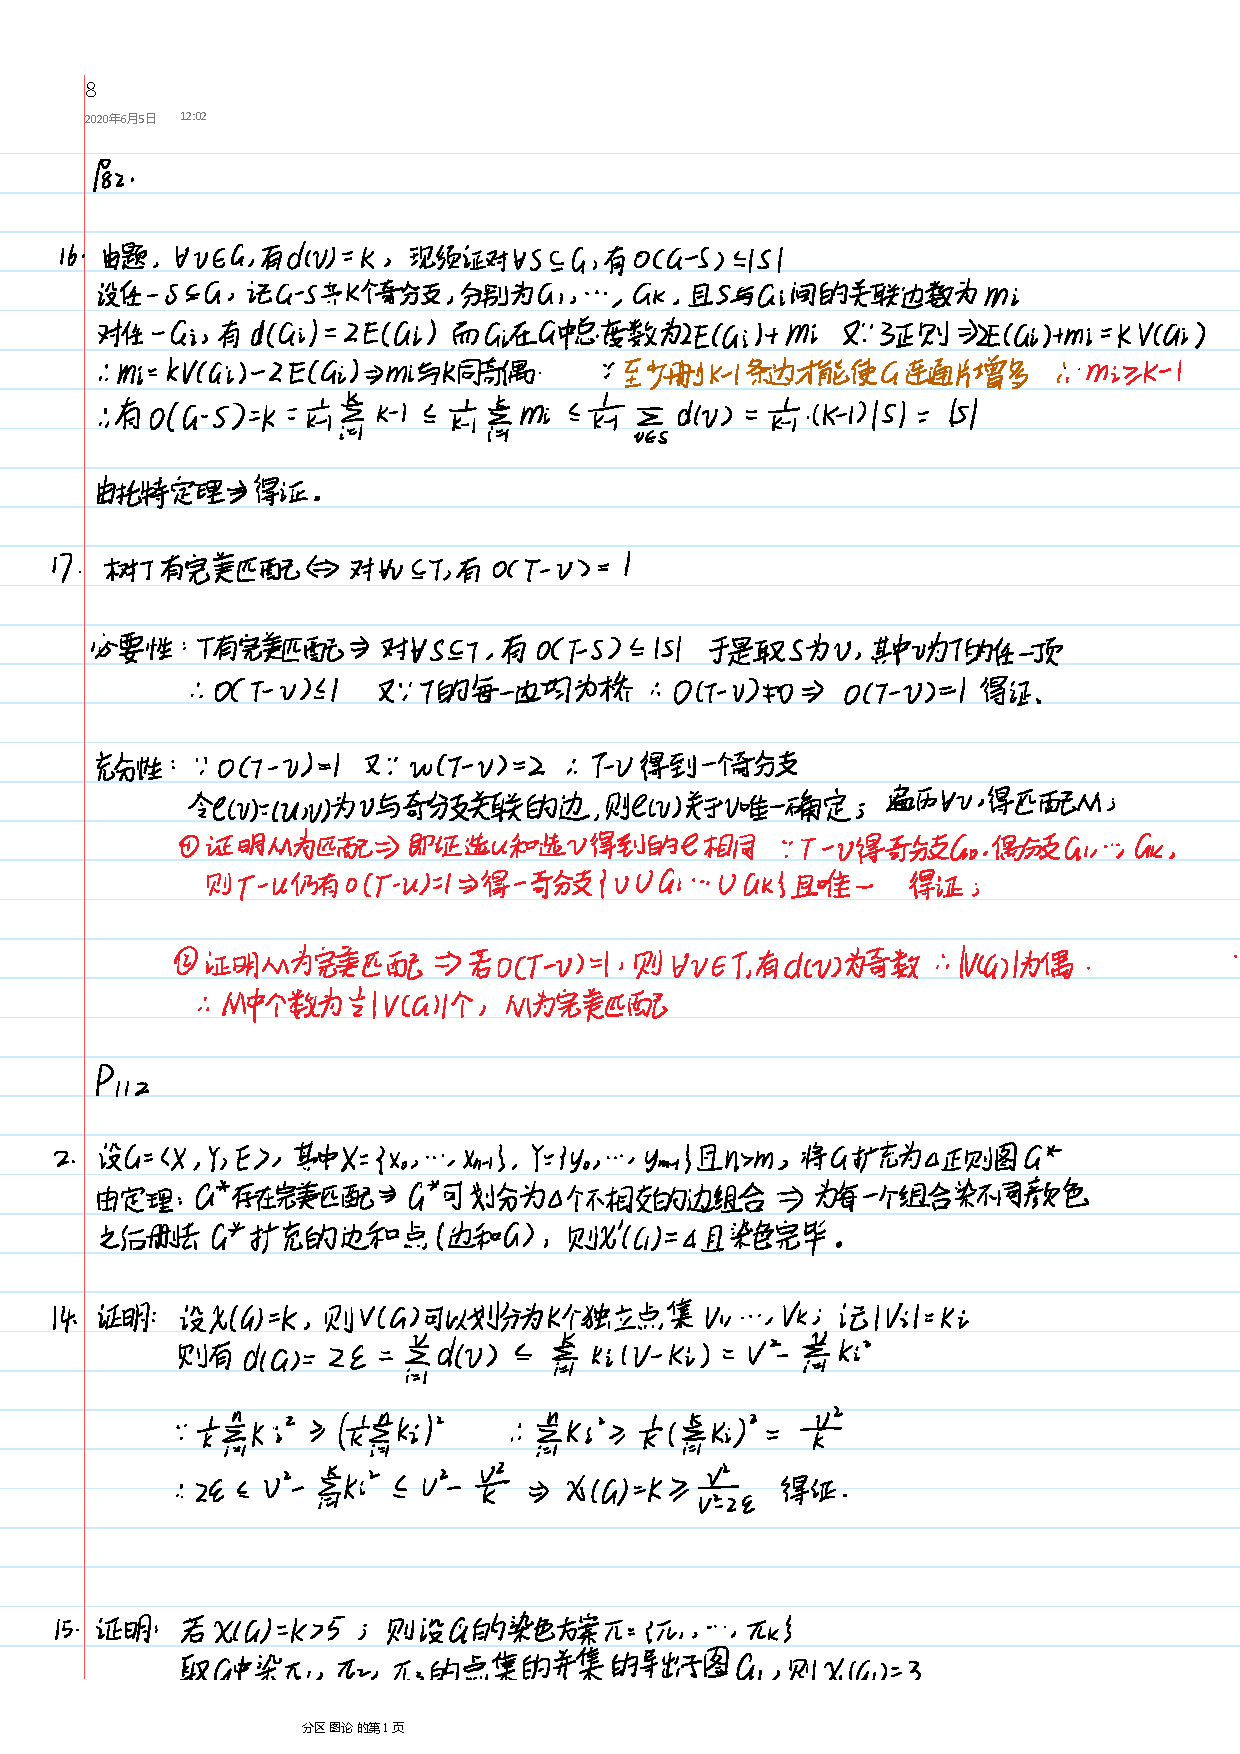
\includegraphics[width=12cm]{resources/9.png}
        \end{figure}
        \item 修改成绩后重新查询,前后对比:
        \begin{figure}
            \centering
            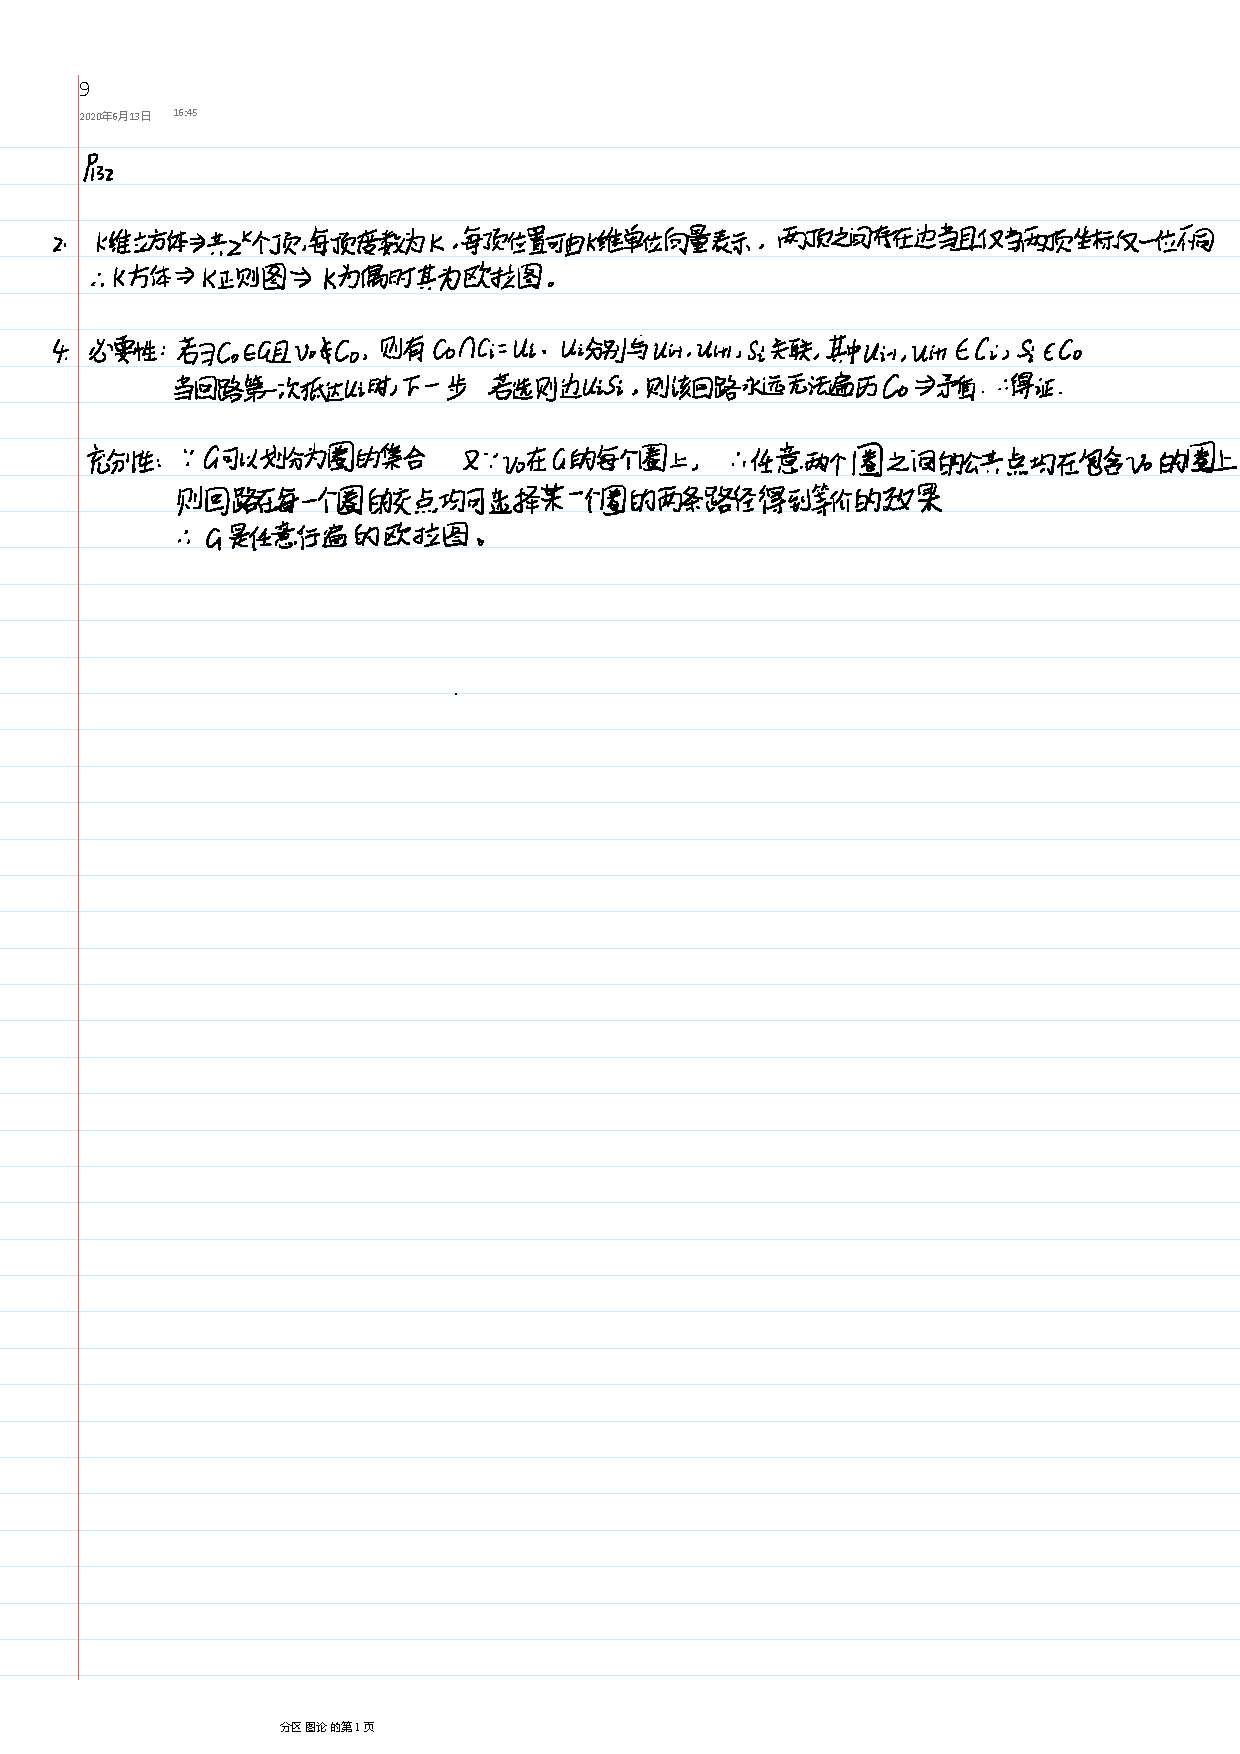
\includegraphics[width=12cm]{resources/10.png}
        \end{figure}
    \end{enumerate}
    \section{实验心得}
    \begin{itemize}
        \item 四个字典中,\textbf{数据有冗余}:学生字典和课程字典中均有某一名学生对某一个课程的成绩,但是这些空间的牺牲导致了更快的查询速度;
        \item 想过\textbf{方法二}:维护两个类(学生、课程)的数个实例和一个矩阵,行为学生,列为课程,矩阵中的值为对应学生和课程的成绩,但这样导致查询某一名学生选修的课程总数和查询某一个课程的选修学生总数代价提升(因为要遍历整个行或列);
        \item 受同学启发想过\textbf{方法三}:使用三元组来存储数据,比如\textbf{学生 -[选修]- 课程},然后维护两个字典,但还没有细想其效率;
        \item 之前对数据库实现的难度没有概念,自己写了之后才发现\textbf{原来这么难,因为要考虑把数据的各个属性都作为键值查询。}但我感觉真正的数据库应该实现地\textbf{又没有数据冗余、又最小化查询代价,}感觉还是很有意思的。
    \end{itemize}
\end{document}